\section{Código Comentado}
\begin{verbatim}
%declarar um objeto modulador PAM
hMod = comm.PAMModulator(2);
%declarar um objeto filtro cosseno levantado
hRCTxFilter = comm.RaisedCosineTransmitFilter(...
'Shape','Normal', ...
'RolloffFactor',0.5, ...
'FilterSpanInSymbols',Rup, ...
'OutputSamplesPerSymbol',Rup);
%taxa de upsampling
Rup = 64;
%número de bits = ndBit
% %para gerar os exemplos com 100 bits fazer ndBit=100 e comentar a parte do código
% %que gera as diferentes BERs
ndBit=100000;
%geração de dados
data = (ones(ndBit,1)+sign(rand(ndBit,1)-0.5))/2;
%convolução dos dados através da resposta do Modulador
modData = step(hMod, data);
%declarar objeto Diagrama de Constelação
hScope = comm.ConstellationDiagram('SamplesPerSymbol',Rup);
%convolução dos dados na saída do PAM através do filtro cosseno levantado
txSig = step(hRCTxFilter,modData);
%ganho casado
gain = 1/max(hRCTxFilter.coeffs.Numerator);
%convolução dos dados na saída do PAM através do filtro casado
txSig = gain*step(hRCTxFilter,modData);
%Diagrama de Constelação sem Ruído
step(hScope,txSig);

%Geração do ruído AWGN
rcv = awgn(txSig,20,'measured');
%Diagrama de Constelação com Ruído
%step(hScope,rcv)
%EbNo, gerar valores de Eb/No entre 0.1 e 10 em incrementos de 0.1
EbNo=[0.1:100]/10;
%variável auxiliar de contagem de erros
c=0;
for a=1:100
%gerar novo ruído AWGN para EbNo(a)
    arcv=awgn(txSig,EbNo(a),'measured');
%trazer o ruído gerado para cada bit
    arcvd=downsample(arcv,Rup);
%recuperar os dados
    txSigD=downsample(txSig,Rup);
    for b=1:ndBit
    %lógica símples de contador
        if txSigD(b)>0
            if arcvd(b)<0
                c =c+1;
            end
        end
        if txSigD(b)<0
            if arcvd(b)>0
                c =c+1;
            end
        end
    end
    %cálculo da ber para 100000 pontos
    ber100k(a)=c/ndBit
    c=0;
end


%cálculo da BER para 10000 pontos, mesma lógica que o laço anterior
ndBit2 = 10000;
data2 = (ones(ndBit2,1)+sign(rand(ndBit2,1)-0.5))/2;
modData2 = step(hMod, data2);
gain2 = 1/max(hRCTxFilter.coeffs.Numerator);
txSig2 = gain2*step(hRCTxFilter,modData);
for a=1:100
    arcv=awgn(txSig2,EbNo(a),'measured');
    arcvd=downsample(arcv,Rup);
    txSigD=downsample(txSig2,Rup);
    for b=1:ndBit2
        if txSigD(b)>0
            if arcvd(b)<0
                c =c+1;
            end
        end
        if txSigD(b)<0
            if arcvd(b)>0
                c =c+1;
            end
        end
    end
    ber10k(a)=c/ndBit2
    c=0;
end

%cálculo da BER para 1000 pontos, mesma lógica dos outros laços
ndBit3 = 1000;
data3 = (ones(ndBit3,1)+sign(rand(ndBit3,1)-0.5))/2;
modData3 = step(hMod, data3);
gain3 = 1/max(hRCTxFilter.coeffs.Numerator);
txSig3 = gain3*step(hRCTxFilter,modData);
for a=1:100
    arcv=awgn(txSig3,EbNo(a),'measured');
    arcvd=downsample(arcv,Rup);
    txSigD=downsample(txSig3,Rup);
    for b=1:ndBit3
        if txSigD(b)>0
            if arcvd(b)<0
                c =c+1;
            end
        end
        if txSigD(b)<0
            if arcvd(b)>0
                c =c+1;
            end
        end
    end
    ber1k(a)=c/ndBit3
    c=0;
end
%geração da figura da BER em escala linear, é preciso editar a figura para mudar
%a escala no eixo das ordenadas
figure; plot(EbNo,ber100k,EbNo,ber10k,EbNo,ber1k);

\end{verbatim}
\section{Constelação}
No caso da geração dos diagramas de constelação, pode-se ver que na medida que a relação sinal ruído se deteriora, a nuvem de pontos em torno de -1 e +1 se torna mais espalhada. Este comportamento se dá devido à distribuição dos pontos de ruído branco. Como o ruído branco é distribuído de forma gaussiana e aditiva com média 0, cada ponto da constelação será deslocado de um certo valor porém mantendo seu centro, de fato se pudéssemos plotar a distribuição de pontos em torno de -1 e +1 veríamos duas gaussianas.
\subsection{Sem Ruído}
\begin{figure}
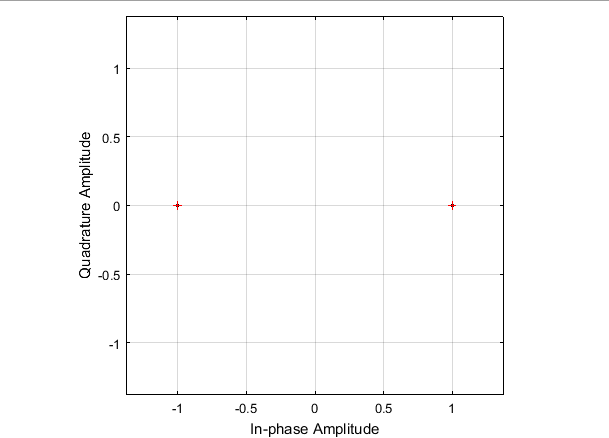
\includegraphics[width=\linewidth]{ConstelaBinSR.png}
\caption{Constelação Obtida sem Ruído}
\end{figure}
\pagebreak
\subsection{Com Ruído}
\begin{figure}
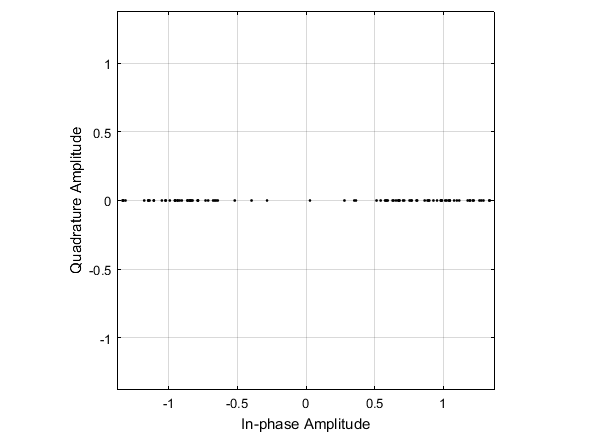
\includegraphics[width=\linewidth]{ConstelaBin10.png}
\caption{Constelação Obtida com Eb/No = 10dB}
\end{figure}
\begin{figure}
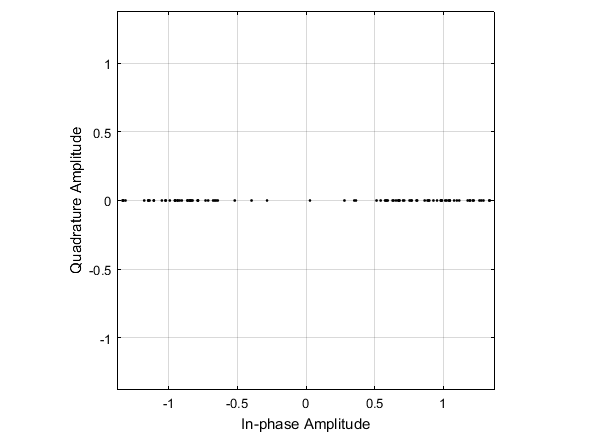
\includegraphics[width=\linewidth]{ConstelaBin10.png}
\caption{Constelação Obtida com Eb/No = 5dB}
\end{figure}
\pagebreak
\section{Taxa de Erro de Bit e Probabilidade de Erro}
É possível ver que para um certo número de bits transmitidos a BER calculada difere um pouco do que seria esperado para a função Q. Este comportamento é esperado pois a natureza estocástica do erro de bit fará com que a medida que aumentamos o número de bits transmitidos usados para calcular a BER, tenhamos um comportamento mais próximo à curva estudada em sala. Em geral temos um pouco mais ou menos erros de bits do que o centro da média que seria a função Q, como transmitimos poucos bits, cada erro terá um peso maior no cálculo da BER, desta forma observamos uma grande flutuação para poucos bits transmitidos e uma flutuação menor para muitos bits pois cada erro individualmente conta menos para o cálculo da BER.\\

É claramente observável que a medida que melhoramos a relação entre a energia transmitida e o ruído, a BER cai. De acordo com o que estudamos em sala.\\
\begin{figure}
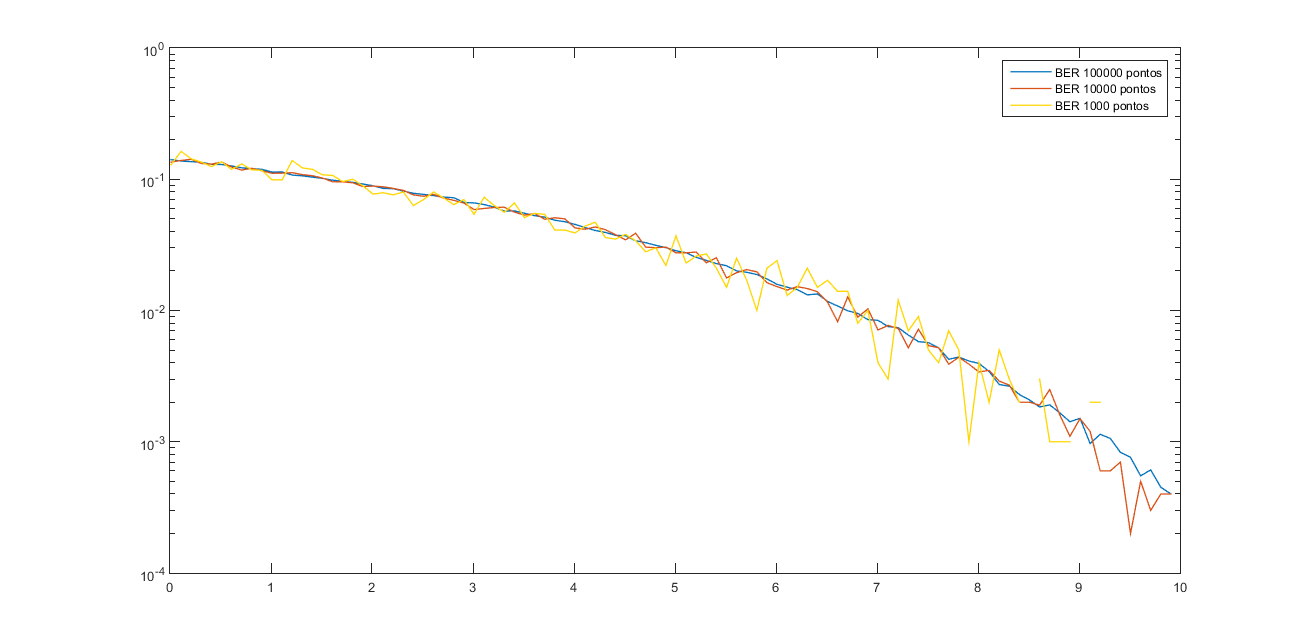
\includegraphics[width=\linewidth]{BERfigura.png}
\caption{Taxas de Erro de Bit para Eb/No em incrementos de 0.1}
\end{figure}